

\documentclass{article}\usepackage[]{graphicx}\usepackage[]{color}
%% maxwidth is the original width if it is less than linewidth
%% otherwise use linewidth (to make sure the graphics do not exceed the margin)
\makeatletter
\def\maxwidth{ %
  \ifdim\Gin@nat@width>\linewidth
    \linewidth
  \else
    \Gin@nat@width
  \fi
}
\makeatother

\definecolor{fgcolor}{rgb}{0.345, 0.345, 0.345}
\newcommand{\hlnum}[1]{\textcolor[rgb]{0.686,0.059,0.569}{#1}}%
\newcommand{\hlstr}[1]{\textcolor[rgb]{0.192,0.494,0.8}{#1}}%
\newcommand{\hlcom}[1]{\textcolor[rgb]{0.678,0.584,0.686}{\textit{#1}}}%
\newcommand{\hlopt}[1]{\textcolor[rgb]{0,0,0}{#1}}%
\newcommand{\hlstd}[1]{\textcolor[rgb]{0.345,0.345,0.345}{#1}}%
\newcommand{\hlkwa}[1]{\textcolor[rgb]{0.161,0.373,0.58}{\textbf{#1}}}%
\newcommand{\hlkwb}[1]{\textcolor[rgb]{0.69,0.353,0.396}{#1}}%
\newcommand{\hlkwc}[1]{\textcolor[rgb]{0.333,0.667,0.333}{#1}}%
\newcommand{\hlkwd}[1]{\textcolor[rgb]{0.737,0.353,0.396}{\textbf{#1}}}%

\usepackage{framed}
\makeatletter
\newenvironment{kframe}{%
 \def\at@end@of@kframe{}%
 \ifinner\ifhmode%
  \def\at@end@of@kframe{\end{minipage}}%
  \begin{minipage}{\columnwidth}%
 \fi\fi%
 \def\FrameCommand##1{\hskip\@totalleftmargin \hskip-\fboxsep
 \colorbox{shadecolor}{##1}\hskip-\fboxsep
     % There is no \\@totalrightmargin, so:
     \hskip-\linewidth \hskip-\@totalleftmargin \hskip\columnwidth}%
 \MakeFramed {\advance\hsize-\width
   \@totalleftmargin\z@ \linewidth\hsize
   \@setminipage}}%
 {\par\unskip\endMakeFramed%
 \at@end@of@kframe}
\makeatother

\definecolor{shadecolor}{rgb}{.97, .97, .97}
\definecolor{messagecolor}{rgb}{0, 0, 0}
\definecolor{warningcolor}{rgb}{1, 0, 1}
\definecolor{errorcolor}{rgb}{1, 0, 0}
\newenvironment{knitrout}{}{} % an empty environment to be redefined in TeX

\usepackage{alltt}
\usepackage[margin=1in]{geometry}
\usepackage{graphicx}
\usepackage{wrapfig}
\IfFileExists{upquote.sty}{\usepackage{upquote}}{}
\begin{document}
\title{Group Project \\ Framingham Heart Study}
\author{Arvind Ramakrishnan \\ Eric Reed \\ Sangsoo Park}
\maketitle
\tableofcontents
\write18{wget https://github.com/arvindram12/Final-Project/blob/master/Rplot01.png}
\newpage





\section{Characteristics of the Data Set}

  This data set is the result of the Framingham Heart Study, which was performed to identify the main risk factors for Cardiovascular Disease (CVD).  The study began in 1948, and recruited individuals from Framingham, Massachusetts. More information about the study can be found at their website at http://www.framinghamheartstudy.org/. 

\subsection{Observations}

In total the data set contained 11,627 observations. However, there were multiple observations made for each individual in the study, as was evident that multiple observations had the same ID number.  Therefore, we filtered the data to include just the first observation for each study participant. We are left with one observation for each of the 4,434 study participants.





\subsection{Variables}

In total, the data set is comprised of 39 variables, of which our analysis will focus on 13. Of these 13 variables 8 are continuous and 5 are categorical.  Summary statistics of all variables are demonstrated in Table 1.

\begin{table}[ht]
\begin{scriptsize}
\centering
\begin{tabular}{rllllll}
  \hline
 Continuous Variables &  &  &  &  & \\ 
 \hline
    & Unit & Mean & Standard Deviation & Median & No. Missing   \\ 
   Total Cholesterol & $mg/dl$ &  236.98 & 44.65 & 234 & 52    \\ 
   Age & $years$ & 49.93 & 8.68 & 49 & 0   \\ 
   Systolic Blood Pressure & $mm Hg$ & 132.91 & 22.42 & 129 & 0   \\ 
   Diastolic Blood Pressure & $mm Hg$ & 83.08 & 12.06 & 82 & 0  \\ 
   Cigarettes Per Day & $quantity$ & 8.97 & 11.93 & 0 & 32  \\ 
  Body Mass Index & $kg/m^2$ & 25.85 & 4.10 & 25.45 & 19   \\ 
 Heart Rate & $beats/min$ & 75.89 & 12.11 & 75 & 1  \\ 
   Glucose Level & $mg/dL$ & 82.19 & 24.40 & 78 & 397   \\ 
    \hline
   Categorical Variables & & & &  & \\ 
    \hline
    & Male & Female & No. Missing & &  \\ 
   Sex & 43.84\% & 56.16\% & 0 & &\\ 
   \hline
   & No & Yes & No. Missing & &  \\ 
   Smoking Status & 50.81\% & 49.19\% & 0 & &  \\ 
   Diabetes Status & 97.27\% & 2.73\% & 0 & &  \\ 
   Blood Pressure Med. Status & 96.71\% & 3.29\% & 61 & &   \\ 
   \hline
   &  Gr. 1-11 & HS Diploma/GED &  Some College & College Degree & No. Missing \\ 
   Education & 43.17\% & 29.65\% & 16.57\% & 11.62\% & 113 \\ 
   \hline
\end{tabular}
\caption{Summary Statistics of 13 Variables in the Framingham Heart Study}
\end{scriptsize}
\end{table}

\subsubsection*{Continuous Variables}

The study participants ranged in age from 32 to 70-years-old, with a mean of 49.94-years-old.

To demonstrate symmetry, the median as well as mean was given in table 1.  All continuous variables had reasonable symmetry, with relatively close mean and medians, except for the data for the number of cigarettes smokes per day.  In this case the mean was 8.97, while the median was 0.  This is consistent with the smoking status, variable that more than half of the participants are non-smokers.

\subsubsection*{Categorical Variables}

The data demonstrates that the study included a close-to equal number of men and women, 43.84\% and 56.16\% respectively, as well as the number of non-smokers to smokers, 50.81\% and 49.19\% receptively.  Diabetes status and blood pressure medication status, showed a much greater departure from equality, and over 95\% in each were of negative status. Interestingly, almost half, 43.17\%, of the participants did not have a high school diploma.   






\subsection{Missing Data}




Of the 4434 observations in our data set, 3,826 of them have complete data. We are missing 52 observations for total cholesterol, 32 observations for cigarettes per day, 19 observations for BMI, 61 observations for blood pressure medication, 1 observation for heart rate, 397 observations for glucose, and 113 observations for education.

\subsection{Candidate Continuous Variables for Linear Regression}

\begin{table}[h]
\centering
\begin{tabular}{rrrrrrrrr}
  \hline
 & TOTCHOL & AGE & SYSBP & DIABP & CIGPDAY & BMI & HEARTRTE & GLUCOSE \\ 
  \hline
TOTCHOL & 1.00 & & & & & & & \\ 
  AGE & 0.25 & 1.00 & & & & & & \\ 
  SYSBP & 0.21 & 0.40 & 1.00 & & & & & \\ 
  DIABP & 0.17 & 0.20 & 0.78 & 1.00 & & & & \\ 
  CIGPDAY & -0.03 & -0.19 & -0.10 & -0.06 & 1.00 & & & \\ 
  BMI & 0.12 & 0.13 & 0.32 & 0.38 & -0.10 & 1.00 & & \\ 
  HEARTRTE & 0.10 & -0.01 & 0.18 & 0.19 & 0.07 & 0.08 & 1.00 & \\ 
  GLUCOSE & 0.05 & 0.12 & 0.13 & 0.05 & -0.06 & 0.09 & 0.09 & 1.00 \\ 
   \hline
\end{tabular}
\caption{Correlation Matrix of 8 Continuous Variables in the Framingham Heart Study}
\end{table}

\begin{wrapfigure}{r}{0.5\textwidth}
  \begin{center}
    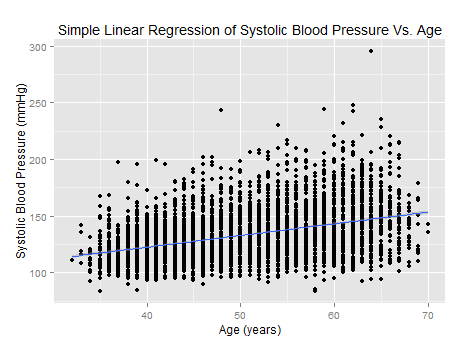
\includegraphics[width=0.4\textwidth]{Rplot01.png}
  \end{center}
  \caption{Association between Systolic Blood Pressure and Age}
\end{wrapfigure}

From the figure we can see that the most consistent correlation between one variable and the others appears to be Systolic Blood pressure.  This is a good outcome variable because it intuitively makes sense as an outcome, whereas other variables such as BMI occur in a large part due to environmental and lifestyle factors that aren't factored into this study, such as diet. Systolic Blood Pressure has the strongest correlation with diastolic blood pressure, however this is an irrelevant relationship to study as it they are virtually always measured at the same time. 

The second highest correlation is between age and systolic blood pressure, $\rho=0.40$.  This makes intuitive sense, since increasing age and systolic blood pressure, can both be attributed to degrading health throughout the lifespan.  A plot of systolic blood pressure vs. age is demonstrates in figure 1.  The equation for this regression model is $\hat{Y}=81.50+1.03X_i$, and has a $R^2$ value of 0.16.   Despite having the highest correlation, the level of variation of systolic blood pressure that can be attributed to age is still relatively low. Throughout the following analyses we will attempt to demonstrate strategies for building models that will contribute better predictive value for systolic blood pressure.

\section{Model Selection}

\subsection{Introduction}

  The purpose of this analysis is to utilize three model selection metrics, Adjusted $R^2$, Aikake Information Criterion(AIC), and Bayesian information criterion (BIC), to explore how choice of these criterion can impact model selection. We will due this by building different Multiple Linear Regression Models of different combinations of predictor variables on the outcome variable, assuming linear relationships of each variable and outcome variable.  The outcome variable being estimated was systolic blood pressure.  Every model included age and sex of the study participants. The continuous variables being tested were, total cholesterol, body mass index, blood pressure, and glucose level.  The categorical variable being tested for was current smoking status, diabetes status, whether or not the participants takes blood pressure medication, and education level.

\subsubsection*{Adjusted $R^2$}
  Adjusted $R^2$ is a selection metric that using the equation: $$R^2_a = 1-\frac{RSS/(n-p-1)}{TSS/(n-1)}$$.  Where $RSS$ is the residual sum of squares of the predictor variables, $TSS$ in the total sum of squares of the  outcome variable, $p$ is the number of predictor variables and $n$ is the number of observations.  This metric is comparable to a typical $R^2$ calculation which is simply $$R^2=1-\frac{RSS}{TSS}$$.  What makes adjusted $R^2$ more suitable for model selection testing however, is that it may penalize added variables that don't contribute predictive value to the model.  Predictive value of a model is assigned via, Adjusted $R^2$, through a resulting value's closeness to 1.
\subsubsection*{Aikake Information Criterion}
 The equation for Aikake Information Criteria is $$ AIC=nlog(RSS/n)+2(p+1)$$.  As with adjusted $R^2$, it includes the variable for residual sum of squares, number of variables and number of observations.  As is evident by apparent differences between the two equations, the AIC uses a different algorithm, and therefore measures predictive value differently.  However, it functions similarly that it penalizes higher values for residual sum of squares of the predictor variables and for added variable.  Also, counter to adjusted $R^2$, lower values of AIC are indicative to increased model predictive value.
 \subsubsection*{Bayesian Information Criterion}
 The equation for Bayesian information criterion is very similar to AIC. It is $$ BIC=nlog(RSS/n)+(p+1)log(n) $$.  Here the equation are identical except for $2(p+1)$ in AIC is replaced with $(p+1)log(n)$.  Here we can see that the two metrics handle the number of observations differently.  They  yield values that are close together, relative to the adjusted $R^2$ model.
 
\subsection{Methods}
This analysis included 8 variables, tested along with sex and age for predictive value of systolic blood pressure.  This results in 255 ($2^8-1$) possible combinations of variables, and therefore 255 possible multiple linear regression models, assuming linearity of every predictor variable.  These models were generated in R using the lm() function.Lists of variables and adjusted $R^2$ were extracted directly from ``lm()" object and AIC and BIC values were calculated for each model using the ``aic()" and ``bic()" functions. respectively. As mentioned before, higher adjusted $R^2$ values and lower AIC and BIC values are indicative to model predictive value. Since, the lm() function by default will omit observations with missing variables, models that include variables with high missing values, such as glucose, will be evaluated with fewer observations.

\subsection{Results and Discussion}

\begin{figure}[h]
\begin{center}
    \centering
    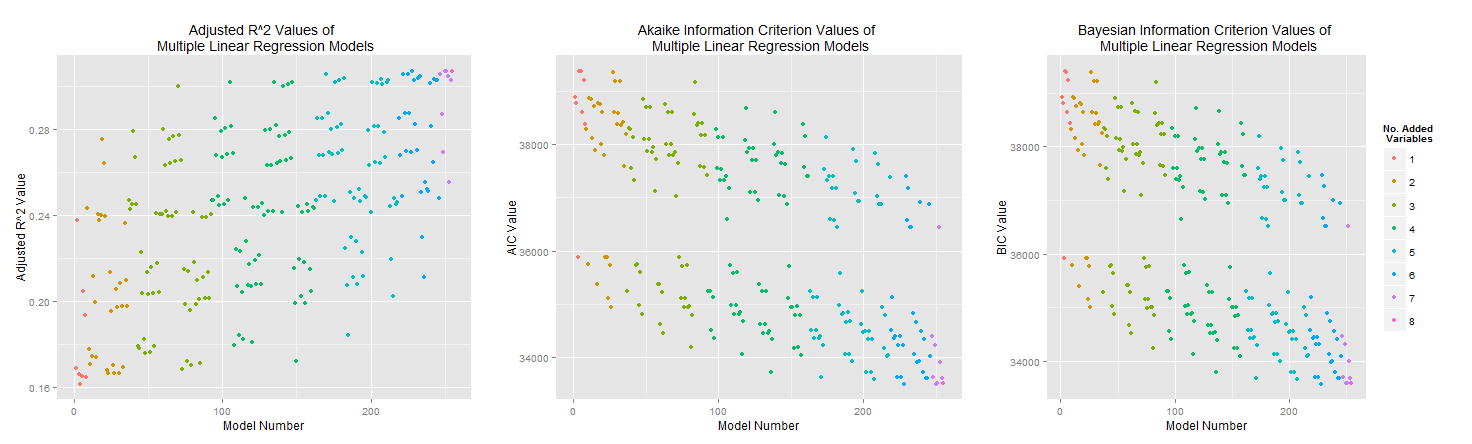
\includegraphics[width=1\textwidth]{3crits.png}
    \caption{Metric Values of MLR Models, Using Three Different  Model Selection Metrics}
    \label{fig:awesome_image}
\end{center}
\end{figure}
  
  Figure 2 depicts the output of each selection metric.  The $x-axis$ represents each of the 255 models that were generated, and the $y-axis$ represents the respective metric value of each model.  Here we can tell that there is a broad trend for predictive value to increase as the number of added variables to increase.  However, we can see that the distribution of the adjusted $R^2$ is very different when compared to that of AIC, BIC. Since the scale of each output is different across the three algorithms, it is difficult to interpret directly how the different selection metrics have ranked the models differently by there values alone. 
  
\begin{figure}[h]
\begin{center}
    \centering
    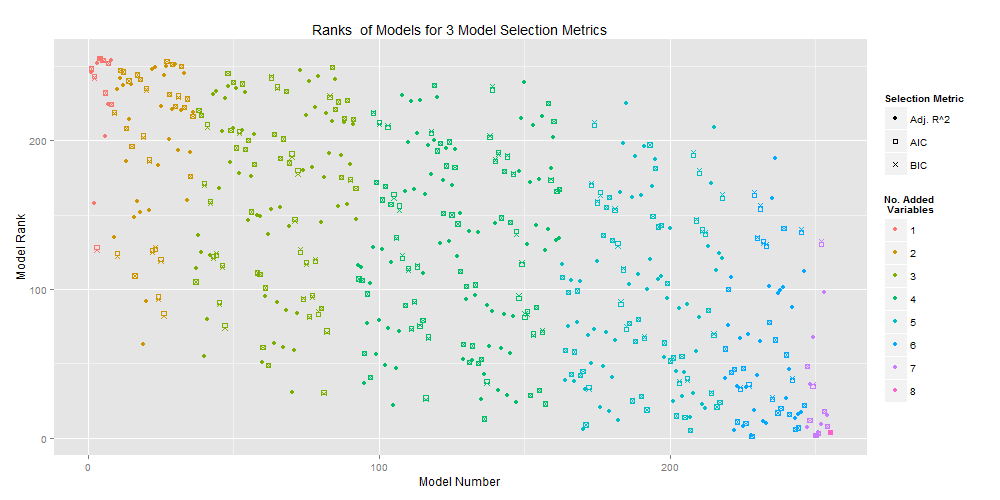
\includegraphics[width=0.8\textwidth]{rank1.png}
    \caption{Ranks of MLR Models, Using Three Different  Model Selection Metrics}
    \label{fig:awesome_image}
\end{center}
\end{figure}  
  Figure 3 represents the ranking of each model, according to each of the three selection metrics. The values of each output are ordered from strongest predictive values, 1, to weakest predictive value, 255.  Since these ranks are on the same scale we can represent all three selection metrics are now interpret table on the same graph.  The most important point here is that each metric can assign a different rank of predictive value to the same model, though AIC and BIC will more often return the same rank for a given model.

Table 3 represents the strongest predictive value for each of the number of added variables using adjusted $R^2$. Table 2 represents the strongest predictive value for each of the number of added variables using AIC and BIC.  AIC and BIC are included in the same table as they agreed on the highest ranked model for each case. In each table the values of the other metric is given as well. 

 



\begin{table}[ht]
\begin{tiny}
\centering
\begin{tabular}{rrllllllllrrr}
  \hline
Variables & Model & Adj $R^2$ & AIC$*10^{-5}$ & BIC$*10^{-5}$ \\ 
  \hline
        1 & BMI & 0.23797 & 0.38773 & 0.38805 \\ 
     2 & BMI+BP Medication & 0.27538 & 0.38006 & 0.38044 \\ 
     3 & BMI+BP Medication+Heart Rate & 0.30014 & 0.37845 & 0.37889 \\ 
     4 & BMI+BP Medication+Heart Rate+Total Chol. & 0.30188 & 0.37398 & 0.37449 \\ 
     5 & BMI+BP Medication+Heart Rate+Total Chol.+Glucose& 0.30543 & 0.34398 & 0.34445 \\ 
     6 & BMI+BP Medication+Heart Rate+Total Chol.+Glucose+Education& 0.30700 & 0.33499 & 0.33575 \\ 
     7 & BMI+BP Medication+Heart Rate+Total Chol.+Glucose+Education+Smoke?& 0.30713 & 0.33500 & 0.33581 \\ 
     8 & BMI+BP Medication+Heart Rate+Total Chol.+Glucose+Education+Smoke?+Diabetes& 0.30700 & 0.33502 & 0.33590 \\  
   \hline
   \end{tabular}
\caption{Multiple Linear Regression Models for Maximum Adjusted $R^2$}
\end{tiny}
\end{table}

   \begin{table}[ht]
   \begin{tiny}
\centering
\begin{tabular}{rrlllllllllrr}
  \hline
  Variables & Model & Adj $R^2$ & AIC$*10^{-5}$ & BIC$*10^{-5}$ \\ 
  \hline
  1 & Glucose & 0.16643 & 0.35880 & 0.38911 \\ 
     2 & Glucose+Education & 0.17036 & 0.34944 & 0.34995 \\ 
     3 & Glucose+Education+BP Medication & 0.21828 & 0.34180 & 0.34236 \\ 
     4 & Glucose+Education+BP Medication+BMI & 0.28165 & 0.33721 & 0.33783 \\ 
     5 & Glucose+Education+BP Medication+BMI+Heart Rate & 0.30299 & 0.33595 & 0.33664 \\ 
     6 & Glucose+Education+BP Medication+BMI+Heart Rate+Total Chol. & 0.30700 & 0.33499 & 0.33575 \\ 
     7 & Glucose+Education+BP Medication+BMI+Heart Rate+ Total Chol.+Smoke? & 0.30713 & 0.33500 & 0.33581 \\ 
     8 & Glucose+Education+BP Medication+BMI+Heart Rate+Total Chol.+Smoke?+Diabetes & 0.30700 & 0.33502 & 0.33590 \\ 
   \hline
\end{tabular}
\caption{Multiple Linear Regression Models for Minimum AIC and BIC}
\end{tiny}
\end{table}

The main trend that every metric followed was that once a variable was added to the model, it was present in each of the following models, when a new variable was added.  For example, in the case of adjusted $R^2$, BMI was demonstrated to be the best single added variable predictor. Next, blood pressure medication status was added along with BMI to be the strongest two added variable predictors.  These two were also present in the strongest 3 added variable predictors along with heart rate.  

What's perhaps most striking is that if we were to try and use these same variables to predict the strongest model by adding fewer than 6 variables, then adjusted $R^2$ and AIC, and BIC would have yielded different models entirely.  For example the strongest three added variable predictor by adjusted $R^2$ was BMI, blood pressure medication, and heart rate,  while that of AIC and BIC was glucose, education, and blood pressure medication.  This is interesting as glucose and education have the most missing values.   What's interesting about this is that all three selection metrics share three attributes, the number of observations, the number of variables, and the residual sum of squares error. Therefore, this disagreement can either occur as a result of AIC and BIC valuing sample size less, or from the exclusion of total sum of squares in AIC and BIC.

Ultimately, the strongest model as predicted by adjusted $R^2$ differed from AIC and BIC by one variable. The strongest model predicted by adjusted $R^2$, in order of added variables was: BMI, blood pressure medication, heart rate, total cholesterol, glucose, education, and smoking status, while that predicted by AIC and BIC in order of added variables was: glucose, education, blood pressure medication, BMI, heart rate, and total cholesterol. Therefore, the addition of smoking status by adjusted $R^2$ and the lack there of in AIC and BIC is the only difference between the strongest estimated model. 

When observing the relative improvement of adding smoking status to the adjusted $R^2$ model, 0.30700 to 0.30712, and the relative penalty of adding smoking status to the AIC and BIC values, 33499 to 33500 and 33575 to 33581 respectively, we observe that adding smoking status contributes very little value in either direction.  If one is concerned with the efficiency of the number of added variables in the model it is reasonable then to exclude smoking status. This model includes: body mass index, blood pressure medication status, heart rate, total cholesterol, glucose, and education.  This is ideal if one is looking for an efficient model that uses fewer variables to account for the variance in the predictor variable.  It is also reasonable however, to use the model that includes smoking, in that if it depreciates the value of the model, it does so by an arguably negligible amount.
\write18{wget https://github.com/arvindram12/Final-Project/blob/master/Validation.png}
\write18{wget https://github.com/arvindram12/Final-Project/blob/master/Comparison_tee.png}

\section{Regression Tree Analysis}
\subsection{Introduction}

  Regression tree analysis can be used to understand underlying structures of data to predict a continuous outcome variable. The analysis divides data into sub-groups using binary branches, which indicates partitioning of observations of an outcome variable, based on predictor variables. 
  There are two benefits using this analysis. First, results from the analysis are simple to understand. Second, we don't need to assume linear relationships between an outcome variable and predictor variables.

In regression tree analysis splits are made to minimizing the residual sum of squares between $y_i$ and $\hat{y}$ at a node. $$RSS = \sum_{i=1}^{n}(y_i - \hat{y})^2$$. This process is repeated using meaningful predictor variables that can greatly improve accuracy of the tree, until a minimum size of the end sub-groups is reached or no longer improvements in the accuracy of adding splits are shown. Thus, we need to have decision criteria do have proper results without over-fitting the model. More details will be explained in the validation of the result section. 

\subsection{Methods}

  For regression tree analysis we utilize the rpart and rpart.plot packages.  The rpart package contains the rpart() function which will perform the analysis based on an input of variables, while the rpart.plot() function will create the regression tree for visualization. Systolic blood pressure was used as the outcome variable, and the same subset of 10 predictor variables from the model selection analysis was used, i.e. age, sex, body mass index, total cholesterol, heart rate, glucose level, blood pressure medication status, smoking status,and diabetes status. The numbers at the terminal are mean systolic blood pressures of the number of observations falling in each terminal.
  There were no missing values for systolic blood pressure, so all observations are considered for regression tree analysis. Predictor variables with missing data are modified by the rpart function by subsetting each variable individually and keep as much data as possible.
  





  



\subsection{Results and Discussion}

  Similar to adding more variables to a multiple linear regression model, adding more splits to the regression tree analysis results in increase in $R^2$. To avoid this over-fitting problem, we need decision criteria on the appropriate number of splits. The cp indicates complexity parameter that allows us to decide the number of meaningful splits (cost of adding one additional split).To be specific, higher cp values lead to smaller number of splits. To start, the initial complexity parameter, cp value, was set to 0.005, which will result in over-fitting of the data. 
  
  There is a rule to decide the number of splits based on the complexity parameter: 1-SE rule. Based on the rule, we can decide the first largest value of cp when cross validation error is smaller than summation of minimum value of cross validation error and cross validation standard deviation. When there are 11 splits, the summated value is 0.803. The largest cp value when the  cross validation error is smaller than 0.803 was 0.01. Based on this result, pruned tree model was generated. This tree contains 6 splits, and includes the following predictor variables: body mass index, blood pressure medication status, age, and heart rate.
  
We can check what the 1-SE means through several plots. There were plots that show how changes in the cp value affect cross-validate $R^2$ values and cross validation errors. First, we can see the number of splits where the overall $R^2$ value is not increased more by increase in cp values after 6 splits (See Figure 4.Bottom left).Second, after the size of tree is larger than 6, there were no further improvements in the X-val relative error while the cp values increase (See Figure 4.Top and Bottom right). Taken together, six splits based on the 1-SE rule was appropriate (cp=0.01). 
  
\begin{figure}[h]
\begin{center}
    \centering
    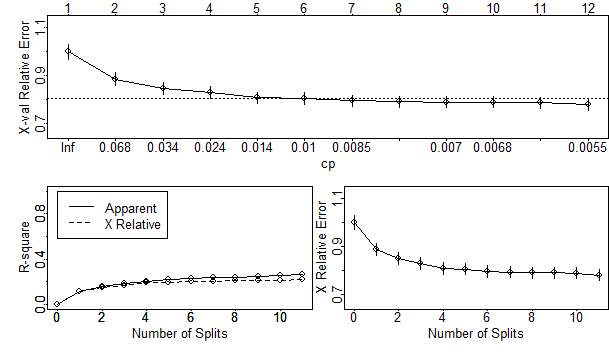
\includegraphics[width=0.6\textwidth]{Validation.png}
    \caption{Decision on the number of splits (Top: X-Val Relative error change as a function of cp, Bottom Right: R-squared value, Bottom left: X Relative Error)}
    \label{Figure 1.}
\end{center}
\end{figure}






  The original tree was pruned based on the 1-SE rule.The original trees used four variables to predict systolic blood pressure with 11 splits. The pruned trees also used the same four variables to predict the outcome variable but it used smaller number of splits (6 splits vs 11 splits).The pruned and the original tree were visualized to see difference between the two trees (See Figure 5).
  
\begin{figure}[ht]
\begin{center}
    \centering
    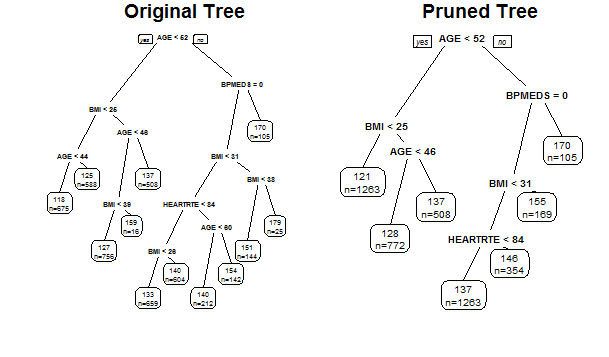
\includegraphics[width=0.8\textwidth]{Comparison_tree.png}
    \caption{Original Tree vs Pruned Tree. Numbers at the terminal nodes indicate mean systolic blood pressure of the number of subjects that is falling into the terminal node, n = number of subjects. If answer to condition in the circle is yes, you can go the left branch.} 
    \label{Figure 2.}
\end{center}
\end{figure}



 

Multiple linear regression analysis was performed with the same variables that the pruned regression tree model used. Results from the multiple regression gives us an idea how an single outcome variable is changed with one unit increase in one of predictor variables while other predictor variables remain constant. It is difficult to visualize the multi-dimensional results and see interactions between the predictor variables.In this context, the benefit of the regression tree model is to have better understanding on data set by binary branches or splits for innate interactions between the predictor variables. Another benefit of the tree model might give us starting point to build reliable multiple regression models. We can add the same predictor variables that the tree model found to build a multiple regression model. The predictor variables in the multiple regression model showed all significant p-values.In terms of accuracy, the multiple linear regression analysis showed higher $R^2$ value, 0.3 as opposed to 0.22 from relative error. This could originate from linear relationships in the data set, which results in higher $R^2$ value from the multiple linear regression model. 




\section{Re-sampling Inference:Bootstrapping}
\subsection{Introduction}


Re-sampling methods (also known as Monte Carlo methods) are a process by which repeated sampling from populations with known characteristics are used to determine how sensitive statistical procedures are to the true population characteristics. An analogy associated commonly with this is that the population is to the sample as the sample is to the bootstrap samples.  The main statistics of interest are typically the mean and variance sample statistics.  Additionally via bootstrapping, confidence intervals of significance can be obtained. \\ 

They are primarily differentiated by whether or not samples are taken with or without replacement.  This section focuses on bootstrapping analysis, which use sampling without replacement to test hypotheses of "no effect", and bootstrap methods, which use sampling with replacement to establish confidence intervals (bootstrap confidence intervals). This is termed case re-sampling and often requires that ${{2n-1) \choose n}}$ based upon the sample size.  This requires extensive computation based on the very large sample size (3,826 individuals) for this analysis.







\subsection{Methods}

To utilize the boot package, all NA values must be removed prior to analysis.  To clean up the data set, the "complete.cases" function was used, which left only 3,826 cases which were used in the bootstrapping analysis.  The presence of NA values causes the boot function to exit and return an NA value.  To ensure the 608 individuals who were not excluded were affecting the data a preliminary correlation analysis was done of the replicates.


\subsubsection*{Re-sampling by Individuals (Rows)}

The first step in bootstrapping is selecting the re-sampling method.  One method occasionally chosen is to randomly select from each variable at the designated sampling rate.  While that method would be suitable if the entire data set were to be used  since then out of the 11,627 observations there would be duplicate patients regardless.  \\

After removing all replicates and even removing all incomplete patient data, we are left with 3,826 observations. This is better for the purposes of the re-sampling inference to compare only these individuals with each other and then compare those with the observations of a patient to compare with the overall populations.  To do this, a correlation analysis was conducted with re-sampling by the individual in the following section.


\subsubsection*{Applying Bootstrapping to Correlations Between Variables}

In bootstrapping confidence intervals, all samples are assumed to be the same and as samples are randomly chosen they are replaced. In this example, the correlation between systolic blood pressure and body mass index between men and women was of interest, and the replacement came from a combined group of the two sets, men and women.  A p-value is determined by the ratio between the count to the number of permutations.

To analyze the effects of re-sampling, consider the obvious correlation between systolic and diastolic blood pressure.  As would be expected, the peak blood pressure of an individual correlates very strongly with the lowest blood pressure of an individual. 

\begin{table}[h]
\begin{small}
    \begin{tabular}{llll}
    \hline \textbf{Data set}             & \textbf{Number of Observations} & \textbf{Correlation} & \textbf{Bias}         \\ \hline
    Original               & 11862              & 0.711       & NA           \\
    One Observation per Participant            & 4434               & 0.7842      & NA           \\ 
    Bootstrapped 1 & R=200              & 0.785       & 6.86 x 10-4  \\
    Bootstrapped 2 & R = 2000           & 0.7849      & -8.93 x 10-5 \\
    \end{tabular}
    \end{small}
\end{table}



To interpret this data, which is outputted by the boot function, the bias is the difference between the mean of the bootstrapped values and the value of the coefficient.  As can be seen above, from the very small bias, the estimated statistic is very close to the true correlation statistic.  This indicates that when re-sampling the complete cases data set with the entire population, the true correlation statistic is very close to the estimator (the bias is the difference between the true statistic and the bootstrap estimate).  








\subsubsection*{Applying Bootstrapping Confidence Intervals to the Multiple Linear Regression Models}

Now that it has been shown that the bootstrapped population of the complete cases is comparable to the entire population of the Framingham Heart Study, bootstrapping analysis can be conducted upon the linear regression models to evaluate our confidence in the predictor variables.

Confidence intervals were obtained using the 'boot' package and quantile functions. Analysis was conducted upon the two best regression models obtained by the model selection methods of analyzing adjusted $R^2$, AIC and BIC which was then compared to linear regression models obtained via the regression trees.  The bootstrap for multiple regression relies on multivariate bootstrap sampling, where each of the predictor variables are re-sampled together. This is why re-sampling inference by the individual is the best choice. It provides accurate and precise measurements of the correlation statistics and sample estimates.

As identified above, the two best models were using six variables via the MLR: body mass index, blood pressure medication status, heart rate, total cholesterol, glucose, and education, and four variables by regression trees: body mass index, age, blood pressure medication status and heart rate.  Additionally the first model also included age and sex, as those are often included in nearly all studies for consistency. 

\subsection{Results and Discussion}
\subsubsection*{Regression models by Regression Trees}

The following is a table of the confidence intervals obtained by bootstrapping the regression tree model using 200 replicates.  It should be noted that due to the vast number of people not taking blood pressure medication (value of 0), NA values were obtained for the confidence interval.  Therefore, it is recommended that the blood pressure medication variable be removed from the prediction for systolic blood pressure.  Overall, we can see that none of the confidence intervals of the coefficients from the regression tree model contain a zero value.  Therefore, they can all be considered a valuable predictor from a bootstrapping analysis predictor for the model.

\begin{table}[h]
\begin{small}
    \begin{tabular}{llll}
    \hline \textbf{Coeff. of the Predictor Variable} & \textbf{ (2.5\%)} & \textbf{Upper Bound (97.5\% )} & \textbf{Coeff. of the Reg. Tree Model}\\ \hline
    Body Mass Index                                  & 0.8877              & 2.609       &   1.5655       \\
    Age                                   & 0.5857              & 1.436        &  1.0973       \\
    Blood Pressure Medication                                & NA                  & NA          & 26.0909         \\
    Heart Rate                              & 0.06611             & 0.7799    &   0.3446         \\
    \end{tabular}
    \end{small}
\end{table}

\

\subsubsection*{Regression model by MLR:}


The following is a table of the confidence intervals obtained by bootstrapping the multiple linear regression model using 200 replicates.  Like in the regression tree model, it should be noted, due to the vast number of people not taking blood pressure medication, value of zero, the confidence interval could not be completed.


\begin{table}[h]
\begin{small}
    \begin{tabular}{llll}
       \hline \textbf{Coeff. of the Predictor Variable} & \textbf{Lower bound (2.5\%)} & \textbf{Upper Bound (97.5\% )} & \textbf{Coeff. from MLR}\\ \hline
    Body Mass Index                                  & 0.6821              & 2.907       &   1.791        \\
    Sex                                   & \textbf{-6.129}              & \textbf{11.08} & 0.5860            \\
    Age                                   & 0.2212              & 1.25        & 0.10123          \\
    Blood Pressure Medication                                & NA                  & NA    & -13.05                \\
    Heart Rate                              & 0.06092             & 0.774       & 0.17321          \\
    Total Cholesterol                                & \textbf{-0.1196}             & \textbf{0.1197}    & 0.0334        \\
    Education                                  & -8.141              & -0.2153     & -7.133          \\
    Glucose                             & \textbf{-0.229}              & \textbf{0.3433}    & 0.0975          \\
    \end{tabular}
    \end{small}
\end{table}

When analyzing the above table it can be seen that sex, total cholesterol, education and glucose level variables all include the zero confidence interval.  This means that there are questions about whether or not they are actually significant predictors.  Additionally, the blood pressure medication variable plays the role of a confounder, similar to the regression tree model and could therefore, possibly be removed without significantly affecting the model.\\

Finally, to compare the model when age and sex are not included the following table is obtained:

\begin{table}[h]
\begin{small}
    \begin{tabular}{llll}
    \hline \textbf{Coeff. of the Predictor Variable} & \textbf{Lower bound (2.5\%)} & \textbf{Upper Bound (97.5 \%)} & \textbf{Coeff. from MLR} \\ \hline
    Body Mass Index             & 0.6969            & 3.197    &    2.5553       \\
    Blood Pressure Medication             & NA               & NA        & NA              \\
    Heart Rate           & \textbf{-0.04025}         & \textbf{0.683}  &      0.2987        \\
    Total Cholesterol       & \textbf{-0.1123}       & \textbf{0.1409}   & 0.1448           \\
    Education            & -10.13             & -2.713    & -5.6361             \\
    Glucose         & \textbf{-0.1751}      & \textbf{0.3955}    & 0.1164             \\
    \end{tabular}
    \end{small}
\end{table}

From the above table, some very interesting results are observed.  Most noticeable is that the total cholesterol's confidence interval just barely does not contain the coefficient obtained via multiple linear regression (0.1448 is the coefficient of the predictor).  This has very interesting results indicating that the confidence interval provided is too narrow, and that is including zero in it. Therefore, total cholesterol should not be included in the model.  Alternatively, this may indicate that age and sex are crucial co-predictors to be used in conjunction with total cholesterol.  Finally, removing blood pressure medication from the model is key to obtaining a better model, since it provides several missing values, especially if the bootstrap replicate selects a population of patients who are all not taking any blood pressure medication.  This will lead to the multiple linear regression also not computing a coefficient and will have no predictive effect on the model.  Therefore, it is not a useful measure when compared to the others, therefore a missing value was not only obtained for the confidence intervals but for the coefficient as well. 

Heart rate was considered to be an especially significant predictor, since the bounds of the confidence interval were extremely similar between the regression tree and  original multiple linear regression model.  The lower bounds were  0.06611 and 0.6092 while the upper bounds were 0.7799 and 0.774 for the regression tree and multiple linear regression model respectively.  However, once age and sex were removed the confidence interval for the heart rate predictor included zero( -0.0403, 0.683).  Therefore, the value of heart rate as a predictor decreased because the confidence interval included zero and from the removal of age and sex it can be inferred that heart rate and age are most useful as co-predictors in conjunction with body mass index.


As can be seen of the original five continuous variables and five categorical variables considered for these models, only four together were found to be conclusively associated with systolic blood pressure in this model:  heart rate, age, body mass index, and education.  


\section{Conclusion}

This study included three analyses on the Framingham Heart Study Data,each offering insight into the manner of building and interpreting models to predict systolic blood pressure, from the remaining variables in the data set.  Multiple linear regression allows for quick and easy model building for this outcome variable.  The main shortcoming of this is that it is impossible to build a perfect model. Thus we rely on assumptions made about the data as a means for going about model building in a systematic way.  This was exemplified through the model selection analysis. By far the most important assumption made in this analysis was linear relationships between all of the variables on systolic blood pressure.  This is a fairly bold assumption, however to test every possible relationship between every variable on systolic blood pressure is impossible. By including specific variables in every model we generate, we've also added a new stipulation to the model building process, not as an assumption, but a means for including variables that are commonly included in similar analyses.  

The strength of this analysis is once we've made assumptions then that one can test out every possible remaining model given a set of variables.  Once we've generated the models, testing their predictive value, via Adjusted $R^2$, AIC, and BIC raise new challenges of model selection, as each assigns relative predictive value of each model differently.  Fortunately, our analysis resulted in convergence in the best predicted models of 6 to 8 added variables. Considering the relive penalties of added or excluding variables for these three models, and favoring models of fewer added variables to build models that have the best predictive value per added variable we conclude that the best model for systolic blood pressure, assuming linearity of every predictor variable on systolic blood pressure includes: age, sex, body mass index, blood pressure medication status, heart rate, total cholesterol, and education, where age and sex were included in every possible model.

Though the multiple linear regression model we generated may be useful, it is hard to interpret, and relies heavily on assumption.  Here lies the strength of regression tree analysis.  Though not usable to make predictions, we can use regression trees to summarize the interactions of the predictor variables on systolic blood pressure, without any assumption of linearity.  By intervening in the parameters of this analysis we were able to control the level of fit, and highlight the splits that best summarize the interaction between the predictor variables on the outcome variables.  Using the 1-SE, rule  we were able to prune an over-fitted regression tree to one of 6 splits and 5 variables: age, body mass index, blood pressure medication, and blood pressure medication status. Note that sex is not included in the regression tree model. Since we are not building a predictive model, there is no precedent to set parameters for model building in this case. The multiple linear regression model also didn't show significant p-value even though the variable was included to construct the model. This fact was consistent with the results from the regression tree model. Significant values for all the four predictor variables were found in the multiple regression model based on on the tree model. This indicated that results from the regression tree model could be a good start to build complex multiple regression models. 

The value of the bootstrapping analysis is that it provided a bridge between understanding the difference in model built by multiple linear regression model selection and the regression tree analysis.  Since we are assuming linearity when building our models to optimized  Adjusted $R^2$, AIC, and BIC values, we are not considering the confidence we have that the coefficients for each variable is accurate, but rather the extent to which they can improve our estimates of systolic blood pressure.  It is not surprising then that when performing an analysis that does not assume linearity, such as regression tree analysis that we see different patterns of important variables.  What bootstrapping does it it then allows us to explore our confidence in the level to which we can expect changes in each variable to affect systolic blood pressure, without having to assume linearity.  This allows us to make generalize able inferences about each variable in a model, having a true relationship on systolic blood pressure.

\end{document}
